\documentclass[a4paper,12pt]{article} 

% First, we usually want to set the margins of our document. For this we use the package geometry.
\usepackage[top = 2.5cm, bottom = 2.5cm, left = 2.5cm, right = 2.5cm]{geometry} 
\usepackage[T1]{fontenc}
\usepackage[utf8]{inputenc}

% The following two packages - multirow and booktabs - are needed to create nice looking tables.
\usepackage{multirow} % Multirow is for tables with multiple rows within one cell.
\usepackage{booktabs} % For even nicer tables.

% As we usually want to include some plots (.pdf files) we need a package for that.
\usepackage{graphicx} 

% The default setting of LaTeX is to indent new paragraphs. This is useful for articles. But not really nice for homework problem sets. The following command sets the indent to 0.
%\usepackage{setspace}
%\setlength{\parindent}{0in}
\usepackage{indentfirst}

% Package to place figures where you want them.
\usepackage{float}

% The fancyhdr package let's us create nice headers.
\usepackage{fancyhdr}

\usepackage{amsmath,amsthm,tikz,caption,karnaugh-map}

% To make our document nice we want a header and number the pages in the footer.

\pagestyle{fancy} % With this command we can customize the header style.

\fancyhf{} % This makes sure we do not have other information in our header or footer.

\lhead{\footnotesize Digital Logic(H): Final Review}% \lhead puts text in the top left corner. \footnotesize sets our font to a smaller size.

%\rhead works just like \lhead (you can also use \chead)
\rhead{\footnotesize Mengxuan Wu} %<---- Fill in your lastnames.

% Similar commands work for the footer (\lfoot, \cfoot and \rfoot).
% We want to put our page number in the center.
\cfoot{\footnotesize \thepage} 

\begin{document}

\thispagestyle{empty} % This command disables the header on the first page. 

\begin{tabular}{p{15.5cm}}
{\large \bf Digital Logic(H)} \\
Southern University of Science and Technology \\ Mengxuan Wu \\ 12212006 \\
\hline
\\
\end{tabular}

\vspace*{0.3cm} %add some vertical space in between the line and our title.

\begin{center}
	{\Large \bf Final Review}
	\vspace{2mm}

	{\bf Mengxuan Wu}
		
\end{center}  

\vspace{0.4cm}

\section{Theory}

\subsection{Binary Number System}

\subsubsection{Analog vs. Digital Signals}

Analog signals change continuously over time. 
They convert information into electric waves of varying amplitude and record exact waveform.

Digital signals are discrete time signals generated by digital modulation. 
They are made by sampling along the wave form.

\begin{center}
	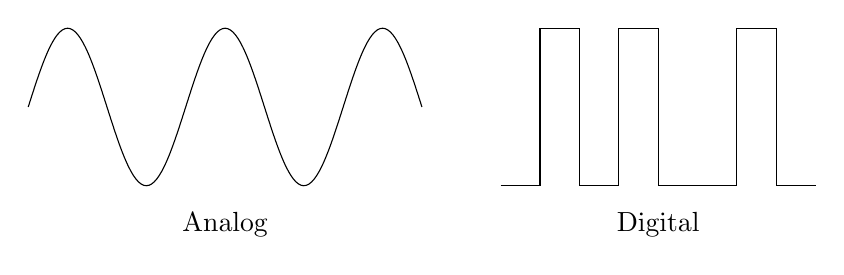
\begin{tikzpicture}
		\draw (0,0) sin (0.5,1) cos (1,0) sin (1.5,-1) cos (2,0) sin (2.5,1) cos (3,0) sin (3.5,-1) cos (4,0) sin (4.5,1) cos (5,0);
		\draw (6,-1) -- (6.5,-1) -- (6.5,1) -- (7,1) -- (7,-1) -- (7.5,-1) -- (7.5,1) -- (8,1) -- (8,-1) -- (8.5,-1) -- (9,-1) -- (9,1) -- (9.5,1) -- (9.5,-1) -- (10,-1);

		\draw (2.5,-1.5) node {Analog};
		\draw (8,-1.5) node {Digital};
	\end{tikzpicture}
\end{center}

A digital system is a system that operates on discrete values and performs operations such as logic, arithmetic, and data storage in a binary format.

\subsubsection{Common Number Systems}

To distinguish different number systems, we use prefix to indicate the base of the number system.
It's common to use ``0'' for octal and ``0x'' for hexadecimal (sometimes ``0b'' for binary).
For example, $(1011)_2 = (11)_{10} = (013)_8 = (0\text{xB})_{16}$.

To convert a number with $n + m$ digits in base $r$ to decimal, we can use the following formula:
\begin{align*}
	D &= \overline{d_{n-1} \cdots d_1 d_0. d_{-1} d_{-2} \cdots d_{-m}} \\
	&= d_{n-1} r^{n-1} + \cdots + d_1 r^1 + d_0 r^0 + d_{-1} r^{-1} + \cdots + d_{-m} r^{-m} \\
	&= \sum_{i=-m}^{n-1} d_i r^i
\end{align*}

\newpage
To convert a decimal number to base $r$, we can use the following algorithm:
\begin{figure}[H]
	\begin{minipage}{0.5\textwidth}
		\centering
		\resizebox{\linewidth}{!}{
		\begin{tabular}{cccc}
			\toprule
			& Quotient & Remainder & Coefficient \\
			\midrule
			$13 \div 2$ & 6 & 1 & $a_0 = 1$ \\
			$6 \div 2$ & 3 & 0 & $a_1 = 0$ \\
			$3 \div 2$ & 1 & 1 & $a_2 = 1$ \\
			$1 \div 2$ & 0 & 1 & $a_3 = 1$ \\
			\bottomrule
		\end{tabular}}
		\caption*{Integer Part}
	\end{minipage}
	\begin{minipage}{0.5\textwidth}
		\centering
		\resizebox{\linewidth}{!}{
		\begin{tabular}{cccc}
			\toprule
			& Integer & Fraction & Coefficient \\
			\midrule
			$0.375 \times 2$ & 0 & 0.75 & $a_{-1} = 0$ \\
			$0.75 \times 2$ & 1 & 0.5 & $a_{-2} = 1$ \\
			$0.5 \times 2$ & 1 & 0 & $a_{-3} = 1$ \\
			\bottomrule
		\end{tabular}}
		\caption*{Fractional Part}
	\end{minipage}
\end{figure}

To be noticed, the coefficients are read in \textbf{different order}.
For the integer part, we read the coefficients from bottom to top.
For the fractional part, we read the coefficients from top to bottom.

Therefore, $(13.375)_{10} = (1101.011)_2$.

\subsubsection{Common Notions}

A \textbf{bit} is a binary digit, which is either 0 or 1.
A \textbf{byte} is a group of 8 bits.

The \textbf{most significant bit} (MSB) is the bit that has the largest value.
The \textbf{least significant bit} (LSB) is the bit that has the smallest value.
This also applies to bytes.

The prefix for bits and bytes are as follows:
\begin{center}
	\begin{tabular}{cccc}
		\toprule
		Power & Meaning & Prefix & Abbreviation \\
		\midrule
		$2^{10}$ & $1024$ & Kilo & K \\
		$2^{20}$ & $1024^{2}$ & Mega & M \\
		$2^{30}$ & $1024^{3}$ & Giga & G \\
		$2^{40}$ & $1024^{4}$ & Tera & T \\
		$2^{50}$ & $1024^{5}$ & Peta & P \\
		$2^{60}$ & $1024^{6}$ & Exa & E \\
		$2^{70}$ & $1024^{7}$ & Zetta & Z \\
		\bottomrule
	\end{tabular}
\end{center}

\subsubsection{Complements}

Two types of complements: $r$'s complement (radix complement) and $(r-1)$'s complement (diminished radix complement).
For example, 9's complement of 1234 is $9999 - 1234 = 8765$, and 10's complement of 1234 is $10000 - 1234 = 8766$.
An easier way to calculate the 10's complement is to add 1 to the 9's complement.

To perform subtraction using complements, we replace the subtraction with addition with this formula:
\begin{align*}
	A - B &= A + (r^N - B) - r^N \\
	&= A + r\text{'s complement of }B - r^N
\end{align*}

\newpage
We demonstrate this with an example:
\begin{figure}[H]
	\begin{minipage}{0.5\textwidth}
		72532 - 3250(10's complement is 96750)
		\centering
		\begin{tabular}{rr}
			$A = $ & 72532 \\
			10's complement of $B = $ & +96750 \\
			\hline
			Sum = & 169282 \\
			Discarding the carry = & -100000 \\
			\hline
			$A - B = $ & 69282
		\end{tabular}
		\caption*{(Discarding the carry when $A \geq B$)}
	\end{minipage}
	\begin{minipage}{0.5\textwidth}
		3250 - 72532(10's complement is 27468)
		\centering
		\resizebox{\linewidth}{!}{
		\begin{tabular}{rr}
			$A = $ & 3250 \\
			10's complement of $B = $ & +27468 \\
			\hline
			Sum = & 30718 \\
			Add ``-'' to 10's complement of the sum = & -100000 \\
			\hline
			$A - B = $ & -69282
		\end{tabular}}
		\caption*{(Add ``-'' to 10's complement of the sum when $A < B$)}
	\end{minipage}
\end{figure}

\subsubsection{Signed Binary Numbers}

We use 2's complement to represent signed binary numbers, by make the MSB the sign bit.
This is because arithmetic operations holds even when we use 2's complement in operations.
The range of a signed binary number is $-2^{N-1}$ to $2^{N-1} - 1$.

To represent a negative number, we first represent the absolute value of the number in binary, then find the 2's complement of the binary number, and finally add a negative sign to the MSB.
For example, $(-105)_{10} = (1101001)_2 = (0010111)_{\text{2's Complement}} = (10010111)_{\text{Signed Binary Number}}$.

\subsubsection{BCD Code}

BCD stands for Binary Coded Decimal.
It is a way to represent decimal numbers in binary.
Number 0 to 9 are represented by 4 bits, and the remaining 6 combinations are invalid.

In BCD addition, we add the two numbers digit by digit.
If the sum is greater than 9, we add 6 to the sum.

BCD subtraction is similar to binary subtraction, we convert the subtrahend to 10's complement and add it to the minuend.

\subsubsection{Gray Code}

Gray code is a binary code where two successive values differ in only one bit.
This is useful in error detection and correction, low power design and Karnaugh maps.

The Gray code for 0-15 is as follows:
\begin{center}
	\resizebox{0.2\textwidth}{!}{
	\begin{tabular}{cc}
		\toprule
		Decimal & Gray Code \\
		\midrule
		0 & 0000 \\
		1 & 0001 \\
		2 & 0011 \\
		3 & 0010 \\
		4 & 0110 \\
		5 & 0111 \\
		6 & 0101 \\
		7 & 0100 \\
		8 & 1100 \\
	    9 & 1101 \\
		10 & 1111 \\
		11 & 1110 \\
		12 & 1010 \\
		13 & 1011 \\
		14 & 1001 \\
		15 & 1000 \\
		\bottomrule
	\end{tabular}}
\end{center}
\subsubsection{Error-Detecting Codes}

A parity bit is a bit added to a string of binary code to ensure that the total number of 1-bits in the string is even or odd.
It can only detect odd number of errors.

\subsection{Boolean Algebra \& Logic Gates}

\subsubsection{Boolean Axioms and Theorems}

\begin{center}
	\begin{itemize}
		\item \textbf{Distribution Laws}
			\begin{align*}
				x(y+z) &= xy + xz \\
				x + yz &= (x+y)(x+z)
			\end{align*}
		\item \textbf{De Morgan's Laws}
			\begin{align*}
				(x+y)' &= x'y' \\
				(xy)' &= x' + y'
			\end{align*}
		\item \textbf{Simplification}
			\begin{align*}
				(x+y')y &= xy \\
				xy' + y &= x + y 
			\end{align*}
	\end{itemize}
\end{center}

\subsubsection{Simplify Boolean Function}

A \textbf{literal} is a variable or its complement.
A \textbf{product term} is a product of literals.
A \textbf{sum term} is a sum of literals.
For example, $x'y'z + x'yz + xy'$ has 8 literals, 3 product terms and 1 sum term.

A \textbf{minterm} is a product term in which each variable appears exactly once in either complemented or uncomplemented form.
A \textbf{maxterm} is a sum term in which each variable appears exactly once in either complemented or uncomplemented form.
Each minterm and maxterm corresponds to a unique row in the truth table. ($M_i = m_i'$)

The value of a minterm is 1 only for the row in which the variables have the values specified by the minterm.
The value of a maxterm is 0 only for the row in which the variables have the values specified by the maxterm.

Canonical forms refer to the sum of minterms and product of maxterms.
We often use $\sum$ to denote sum of minterms and $\prod$ to denote product of maxterms.
Note that $(\sum(a_1, a_2, \cdots, a_n))' = \prod(a_1, a_2, \cdots, a_n)$.

Standard forms refer to the forms that is either SOP or POS.

\subsection{Gate-Level Minimization}

We can use Boolean algebra or Karnaugh maps to simplify Boolean functions.

In Karnaugh maps, minterms are arranged in Gray code order.
Some Karnaugh maps may have don't care conditions, which are represented by ``X''.

The task of simplification is to find the implicants.
A prime implicant is a 1-product term that obtained by combining the maximum possible number of adjacent squares in the map.
A prime implicant is essential if it is the only implicant that covers a particular minterm.

Therefore, the simplification steps are as follows:
\begin{enumerate}
	\item Find all essential prime implicants and cover them.
	\item Find a minimum set of prime implicants that cover all the remaining minterms.
\end{enumerate}

Two typical Karnaugh maps are as follows:
\begin{figure}[H]
	\begin{minipage}{0.5\textwidth}
		\centering
		\begin{karnaugh-map}(label=corner)[4][2][1][$BC$][$A$]
			\manualterms{$m_0$, $m_1$, $m_2$, $m_3$, $m_4$, $m_5$, $m_6$, $m_7$}
		\end{karnaugh-map}
		\caption*{3-Variable Karnaugh Map}
	\end{minipage}
	\begin{minipage}{0.5\textwidth}
		\centering
		\begin{karnaugh-map}(label=corner)[4][4][1][$CD$][$AB$]
			\manualterms{$m_0$, $m_1$, $m_2$, $m_3$, $m_4$, $m_5$, $m_6$, $m_7$, $m_8$, $m_9$, $m_{10}$, $m_{11}$, $m_{12}$, $m_{13}$, $m_{14}$, $m_{15}$}
		\end{karnaugh-map}
		\caption*{4-Variable Karnaugh Map}
	\end{minipage}
\end{figure}

\subsection{Two-Level Implementation}

\subsubsection{Universal Gates}

A universal gate is a gate that can implement any Boolean function without need to use any other gate type.
The NAND gate is a universal gate, and so is the NOR gate.

In NAND circuits, we can implement other gates as follows:
\begin{itemize}
	\item Inverter: $x' = \text{NAND}(x, x)$
	\item AND: $xy = (\text{NAND}(x, y))'$
	\item OR: $x + y = \text{NAND}(x', y')$
\end{itemize}

In NOR circuits, we can implement other gates as follows:
\begin{itemize}
	\item Inverter: $x' = \text{NOR}(x, x)$
	\item AND: $xy = \text{NOR}(x', y')$
	\item OR: $x + y = (\text{NOR}(x, y))'$
\end{itemize}

\subsubsection{NAND and NOR Implementations}

We can implement any Boolean function using only NAND or NOR gates.
If the function is in SOP form, we can use NAND gates.
If the function is in POS form, we can use NOR gates.

The expressions are as follows:
\begin{align*}
	ab+cd &= ((ab+cd)')' \\
	&= ((ab)'(cd)')' \\
	(a+b)(c+d) &= (((a+b)(c+d))')' \\
	&= ((a+b)'+(c+d)')' \\
\end{align*}

\subsubsection{Two-Level Implementations}

There are 16 possible combinations of two-level implementations and 8 of them degenerate to one-level implementations.
The other 8 can be divided into 4 groups:
\begin{itemize}
	\item AND-OR / NAND-NAND => SOP
	\item OR-AND / NOR-NOR => POS
	\item NAND-AND / AND-NOR => AOI (AND-OR-INVERT or Complement of SOP)
	\item OR-NAND / NOR-OR => OAI (OR-AND-INVERT or Complement of POS)
\end{itemize}

\subsubsection{Exclusive-OR Function}

An odd function is a function that is 1 when the number of 1's in the input is odd.
We can use the XOR function to implement an odd function by XORing all the inputs.
Similarly, an even function is a function that is 1 when the number of 1's in the input is even and can be implemented by XORing all the inputs and then inverting the output.

These two functions are useful in error detection (parity check).
For an even parity bit of 3 inputs, we can use $P = x \oplus y \oplus z$.
And for an even parity checker of the same message, we know $C = x \oplus y \oplus z \oplus P$.

\subsection{Combination Logic}

\subsubsection{Combinational Circuits and Sequential Circuits}

A combinational circuit is a circuit whose outputs depend only on the current inputs.
A sequential circuit is a circuit whose outputs depend on the current inputs and the current state (memory elements).

\subsubsection{Analysis Procedure}

\begin{enumerate}
	\item Label all gate outputs that are functions of the input variables only. Determine the functions.
	\item Label all gate outputs that are functions of the input variables and previously labeled gate outputs, and find the functions.
	\item Repeat previous step until all the primary outputs are obtained.
\end{enumerate}

\subsection{Standard Components}

\subsubsection{Decoder}

A decoder is a combinational circuit that converts binary information from $n$ input lines to a maximum of $2^n$ unique output lines.
We may have an enable input to enable the decoder.

There might be inverters on the output lines or the enable input.
If the enable input is inverted, we call it Active Low Enable.

We can use two lower-order decoders with an enable input to implement a higher-order decoder.
But we need to make sure the MSB of the input is connected to the enable input of both decoders.
\subsubsection{Mutiplexer}

A multiplexer is a combinational circuit that selects binary information from one of many input lines and directs it to a single output line.

Likewise, we can use five lower-order multiplexers to implement a higher-order multiplexer.
And the higher bits are connected to the select inputs the last multiplexer.

\subsubsection{Demultiplexer}

A demultiplexer is a combinational circuit that directs a single input line to one of $2^n$ output lines.
A decoder with an enable input can be used as a demultiplexer.

\subsubsection{Encoder}

An encoder is a combinational circuit that performs the inverse operation of a decoder.

To make sure don't care conditions are not encoded, we can use a priority encoder, which has a priority order for the input lines and a valid output indicator.
The truth table of a priority encoder that $D_3$ has the highest priority is as follows:
\begin{center}
	\begin{tabular}{ccccccc}
		\toprule
		\multicolumn{4}{c}{Inputs} & \multicolumn{3}{c}{Outputs} \\
		\cmidrule(lr){1-4} \cmidrule(lr){5-7}
		$D_0$ & $D_1$ & $D_2$ & $D_3$ & $x$ & $y$ & $V$ \\
		\midrule
		0 & 0 & 0 & 0 & X & X & 0 \\
		1 & 0 & 0 & 0 & 0 & 0 & 1 \\
		X & 1 & 0 & 0 & 0 & 1 & 1 \\
		X & X & 1 & 0 & 1 & 0 & 1 \\
		X & X & X & 1 & 1 & 1 & 1 \\
		\bottomrule
	\end{tabular}
\end{center}

\subsubsection{Tri-state Buffer}

A tri-state buffer has truth table as follows:
\begin{center}
	\begin{tabular}{ccc}
		\toprule
		\multicolumn{2}{c}{Inputs} & Outputs \\
		\cmidrule(lr){1-2} \cmidrule(lr){3-3}
		$E$ & $A$ & $Y$\\
		\midrule
		0 & X & Z \\
		1 & 0 & 0 \\
		1 & 1 & 1 \\
		\bottomrule
	\end{tabular}
\end{center}

\subsection{Gate Delays}

The propagation delay is the time required for the output to change after the input changes.

Because of the propagation delay, we may have glitches in the output.
A static 1-hazard is a glitch that the output goes from 1 to 0 and back to 1 when the output should be 1.
A static 0-hazard is a glitch that the output goes from 0 to 1 and back to 0 when the output should be 0.

\begin{center}
	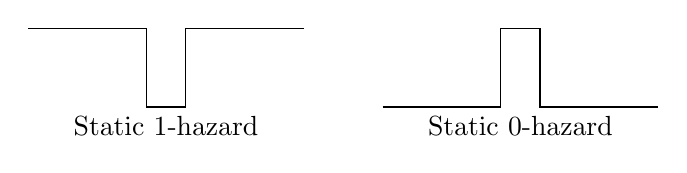
\begin{tikzpicture}
		\draw (-1,1) -- (0.5,1) -- (0.5,0) -- (1,0) -- (1,1) -- (2.5,1);
		\draw (3.5,0) -- (5,0) -- (5,1) -- (5.5,1) -- (5.5,0) -- (7,0);

		\draw (0.75,0) node [below] {Static 1-hazard};
		\draw (5.25,0) node [below] {Static 0-hazard};
	\end{tikzpicture}		
\end{center}

To eliminate glitches, we can use a hazard-free circuit.
If two adjacent minterms in Karnaugh map are always in some prime implicant, we can eliminate the hazard.

For example:
\begin{figure}[H]
	\begin{minipage}{0.5\textwidth}
		\centering
		\begin{karnaugh-map}(label=corner)[4][2][1][$BC$][$A$]
			\minterms{3,4,5,7}
			\autoterms[0]
			\implicant{3}{7}
			\implicant{4}{5}
		\end{karnaugh-map}
		\caption*{With Hazard}
	\end{minipage}
	\begin{minipage}{0.5\textwidth}
		\centering
		\begin{karnaugh-map}(label=corner)[4][2][1][$BC$][$A$]
			\minterms{3,4,5,7}
			\autoterms[0]
			\implicant{3}{7}
			\implicant{4}{5}
			\implicant{5}{7}
		\end{karnaugh-map}
		\caption*{Without Hazard}
	\end{minipage}
\end{figure}

\subsection{Latch and Flip-Flop}

\subsubsection{Latch}

In this course, we only consider SR latch and D latch.
A latch is a sequential circuit that can be in one of two states and can change its state in response to some control inputs.

A SR latch has two inputs: $S$ and $R$.
It usually consists of two cross-coupled NOR gates or NAND gates.
When $S = R = 0$, the latch is in hold state. (The output is the same as the previous state)
When $S = 1$ and $R = 0$, the latch is in set state. ($Q = 1$)
When $S = 0$ and $R = 1$, the latch is in reset state. ($Q = 0$)
When $S = R = 1$, the latch is in invalid state. (Because $Q = Q'$ and this is not possible)

A clocked SR latch has an additional clock input.
We use AND gates to control the inputs of the SR latch.
However, we still might encounter the invalid state when the clock is high and $S = R = 1$.

A D latch has two inputs: $D$ and $C$.
We use an inverters to connect $D$ to $R$ and $S$.
This prevents the invalid state.
When $C = 0$, the latch is in hold state.
When $C = 1$, the latch is in set state if $D = 1$ and reset state if $D = 0$.
D latch is also called transparent latch because the output follows the input when $C = 1$.

A latch is used for level-sensitive control.
But not for edge-sensitive control.

\subsubsection{Flip-Flop}

A flip-flop is a sequential circuit that can be in one of two stable states and can change its state in response to some control inputs.
In this course, we consider D flip-flop, JK flip-flop and T flip-flop.

When we use FF, we must make sure the inputs are stable before the clock rises.
This is called \textbf{setup time}.
And we must make sure the inputs are stable after the clock rises.
This is called \textbf{hold time}.

A D flip-flop is implemented with two D latches.
The first D latch is called master latch, which is negative level triggered.
The second D latch is called slave latch, which is positive level triggered.
The output of the master latch is connected to the input of the slave latch.
When the clock is low, the master latch is enabled and the slave latch is disabled.
When the clock is high, the master latch is disabled and the slave latch is enabled.
This gives us the edge-sensitive control.
The characteristic equation of a D flip-flop is $Q_{n+1} = D$.

A D flip-flop with reset can be implemented in two ways: synchronous reset and asynchronous reset.
A synchronous reset means the value will be reset to 0 at rising edge of the clock.
An asynchronous reset means the value will be reset to 0 immediately when the reset signal is 1.

A JK flip-flop can be implemented with one D flip-flop.
Its characteristic equation is $Q_{n+1} = JQ_n' + K'Q_n$.
When $J = K = 0$, the flip-flop is in hold state.
When $J = 1$ and $K = 0$, the flip-flop is in set state.
When $J = 0$ and $K = 1$, the flip-flop is in reset state.
When $J = K = 1$, the flip-flop is in toggle state.

A T flip-flop can be implemented with one D flip-flop.
Its characteristic equation is $Q_{n+1} = TQ_n' + T'Q_n = T \oplus Q_n$.
When $T = 0$, the flip-flop is in hold state.
When $T = 1$, the flip-flop is in toggle state.

\subsubsection{Excitation Table}

An excitation table is used for designing a sequential circuit.
It tells what inputs are needed when you want particular outputs.
The most important one is the JK flip-flop excitation table.
\begin{center}
	\begin{tabular}{ccccc}
		\toprule
		\multicolumn{2}{c}{Outputs} & \multicolumn{2}{c}{Inputs} & \multirow{2}{*}{Operation} \\
		\cmidrule(lr){1-2} \cmidrule(lr){3-4}
		$Q_n$ & $Q_{n+1}$ & $J$ & $K$ & \\
		\midrule
		0 & 0 & 0 & X & No Change \\
		0 & 1 & 1 & X & Set \\
		1 & 0 & X & 1 & Reset \\
		1 & 1 & X & 0 & Toggle \\
		\bottomrule
	\end{tabular}
\end{center}

\subsection{Synchronous Sequential Circuits}

There are two models for sequential circuits: Mealy model and Moore model.
In Mealy model, the output depends on the current state and the current input.
In Moore model, the output depends on the current state only.

To analyze a synchronous sequential circuit, we can use the following steps:
\begin{enumerate}
	\item Derive the input equations.
	\item Derive state and output equations.
	\item Derive the state and output tables.
	\item Derive the state diagram.
\end{enumerate}

\vspace{1cm}
To design a synchronous sequential circuit, we can use the following steps:
\begin{enumerate}
	\item Derive the state diagram.
	\item Derive the state and output tables.
	\item Minimalize the state table.
	\item Assign binary codes to the states.
	\item Derive the state and output equations.
	\item Choose flip-flops and derive the input equations.
	\item Draw the circuit diagram.
\end{enumerate}

\subsection{Registers and Counters}

\subsubsection{SISO Register}

A serial in, serial out shift register is a register that can shift the data in one bit at a time.
It has one input and one output.
The input is connected to the first flip-flop and the output is connected to the last flip-flop.

\subsubsection{SIPO Register}

This is similar to SISO shift register, we just add an extra wire to each flip-flop to output the data.

\subsubsection{PISO Register}

We use extra combinational logic to control the inputs of the flip-flops.
Usually, it is a MUX to choose from the input and the output of the previous flip-flop.

\subsubsection{PIPO Register}

This is just an array of independent D flip-flops.

\subsubsection{Universal Shift Register}

A universal shift register is a register that can perform all the operations of SISO, SIPO, PISO and PIPO registers.
It has five operations: parallel load, shift left, shift right, hold and reset.

\subsubsection{Serial and Parallel Transfer}

A serial transfer is a transfer that the data is transferred one bit at a time.
A parallel transfer is a transfer that the data is transferred all at once.

We can convert serial transfer to parallel transfer by using a SIPO and PIPO register.

\subsubsection{Sequence Generator}

A sequence generator is a circuit that generates a specified sequence of states.

\section{Lab}

\subsection{Name of Object}

The identifier must begin with an alphabetic character or the underscore character (a-z or A-Z or \_).
Identifiers may contain alphabetic characters, numeric characters, the underscore, and the dollar sign (a-z or A-Z or 0-9 \_ or \$).
That means name like ``1a'' is not allowed.

\subsection{Numbers}

There are four radixes and the syntax should be: <size>'<radix><value>.

The radixes are as follows:
\begin{center}
	\begin{tabular}{cc}
		\toprule
		Radix & Meaning \\
		\midrule
		b & Binary \\
		o & Octal \\
		d & Decimal \\
		h & Hexadecimal \\
		\bottomrule
	\end{tabular}
\end{center}

Value that exceed the size will be truncated.
If the size is omitted, the default size is 32 bits.
For example, ``6’hCA'' is equivalent to ``001010'', and ``hf'' is equivalent to ``00000000000000000000000000001111''.

\subsection{Signed vs. Unsigned}

There are two types of numbers: signed and unsigned.
The default type for integer is signed.
The default type for reg and wire is unsigned.

When we assign a shorter number to a longer number, the shorter number will be extended in two possible ways:
\begin{itemize}
	\item Zero extension: the shorter number is extended with 0's.
	\item Sign extension: the shorter number is extended with the sign bit.
\end{itemize}

\subsection{Wire vs. Reg}

\begin{center}
	\begin{tabular}{cccc}
		\toprule
		Type & Demo & Wire & Reg \\
		\midrule
		Input of a module & module tx(input a) & Yes & No \\
		Output of a module & module tx(output a) & Yes & Yes \\
		Variable in continuous mode & assign a =  & Yes & No \\
		Variable in procedure mode & always @* a = & No & Yes \\
		Variable binds to input port & tx dut(.in(a)) & Yes & Yes \\
		Variable binds to output port & tx dut(.out(a)) & Yes & No \\
		\bottomrule
	\end{tabular}
\end{center}

\subsection{Other Important Facts}

\begin{itemize}
	\item Different size of variables must be declared separately.
	      For example, ``reg [3:0] a, b'' will declare two 4-bit variables.
	\item The type of variable can be declared later in the code.
	      For example, ``output reg [3:0] a'' is equivalent to ``output [3:0] a; reg [3:0] a''.
	\item When using continuous mode, you cannot assign conflicting value to a variable. 
	      For example, ``assign a = 1'b1; assign a = 1'b0;'' is not allowed.
	\item Both structural and data-flow modeling cannot be nested in behavior modeling.
	      For example, ``always @* begin assign a = b; end'' is not allowed.
\end{itemize}
\end{document}